\documentclass{article}
\usepackage{hyperref}
\usepackage{tikz}
\usetikzlibrary{arrows,intersections}
\usetikzlibrary{decorations.markings}

\usepackage{amsmath} % Required for \varPsi below

\hypersetup{
    colorlinks=true,
    linkcolor=blue,
    filecolor=magenta,      
    urlcolor=cyan,
}
\usepackage{graphicx}
\usepackage{float}
\usepackage{rotating}

\begin{document}

\title{Titanic - ML Project}
\author{Bogdanowicz Michal Kamil, Geraci Luca}

\maketitle

\begin{abstract}
Report of the project for the course of ML 2019/2020.
\break The models used are Logistic Regression, Neural networks, Decision trees, Random forests and Naive Bayes Classifier.
\end{abstract}


\section{Proposition}
The proposition is using a set of machine learning methods to predict the people that would survive the Titanic sinking of 15 April 1912.

The methods that have been used are:

\begin{enumerate}  
\item Logistic Regression
\item Neural Networks
\item Decision trees and Random Forest
\item Naive Bayes Classifier
\end{enumerate}

\section{Data}
\subsection{Incomplete Data}

The Data propsed to the professor was incomplete. It heavily reduced the avialble data to perform the best practices for evaluating a model. The test and training were already separated and ground truth was missing. So the complete dataset has been taken from the internet. In addition the complete list of surviors can be found at the wikipedia page \href{https://en.wikipedia.org/wiki/Passengers_of_the_RMS_Titanic}{here} (not a ML-friendly format).
This data sadly is used to cheat on the kaggle competition. Making it a quite infamous one.

\subsection{Data Format}

\begin{itemize}
\item Ticket class
\item Survival 
\item Name
\item Sex
\item Age in years
\item sibsp : number of siblings / spouses aboard the Titanic <-- This might be problematic as it doesn't seem to make much sense.
\item parch : number of parents / children aboard the Titanic<-- This might be problematic as it doesn't seem to make much sense.
\item Ticket number	
\item Fare
\item Cabin/s assigned
\item Port of Embarkation	
\item Rescue Boat
\item Body
\item Destination
\end{itemize}

With additional notes of :
Ticket class: A proxy for socio-economic status (SES)
1st = Upper
2nd = Middle
3rd = Lower

age: Age is fractional if less than 1. If the age is estimated, is it in the form of xx.5

sibsp: The dataset defines family relations in this way
Sibling = brother, sister, stepbrother, stepsister
Spouse = husband, wife (mistresses and fiancés were ignored)

parch: The dataset defines family relations in this way
Parent = mother, father
Child = daughter, son, stepdaughter, stepson
Some children travelled only with a nanny, therefore parch=0 for them.



\subsection{Data Preparation}
The data cannot be used as it is.
The names are going to be deleted, as that should not inlfuence the resut.

\section{Logistic Regression}
\subsection{Remark}

Since a lot of the data is a binary variable (0,1). The square of 0 and 1 comes back to the same value. That means that eleveting features which have only values 0 and 1 adds nothing to the model. Even more, it adds a fully correlated feature. Which has a negative impact on the model (even though it has not been the case empirically for this model. The reasons seems to be that the ensuring overestimation has no effect on the final result. The reasoning used still stands : Avoid correlated features for ML).
\\
\subsection{Procedure}

Procedure used for selecting the Logistic Regression model.

\begin{enumerate}  
\item Tthe maximum polynomial wase chosen by comparing the measures obtained with Cross Valdation (CV) methodology. The data can be seen in Table
\ref{tab:LR-Measures}. Maximim degree 2 has prevailed in most iterations. At each iteration the folds are randomized, and maximum degree 1 rarely beat 2.

\begin{table}[]
\centering
\caption{Polynomial degree measures comparison}
\label{tab:LR-Measures}
\begin{tabular}{|l|l|l|l|l|l|}
\hline
Measure/Degree  & 1     & \textbf{2}     & 3     & 4     & 5     \\ \hline
Accuracy  		& 0.804 & \textbf{0.810} & 0.717 & 0.662 & 0.437 \\ \hline
Precision		& 0.754 & \textbf{0.760} & 0.683 & 0.631 & 0.399 \\ \hline
Recall    		& 0.728 & \textbf{0.738} & 0.436 & 0.286 & 0.896 \\ \hline
F1        		& 0.738 & \textbf{0.746} & 0.515 & 0.390 & 0.534 \\ \hline
MAE       		& 0.196 & \textbf{0.190} & 0.283 & 0.338 & 0.563 \\ \hline
MSE       		& 0.196 & \textbf{0.190} & 0.283 & 0.338 & 0.563 \\ \hline
RAE       		& 0.414 & \textbf{0.403} & 0.599 & 0.715 & 1.193 \\ \hline
RSE       		& 0.828 & \textbf{0.806} & 1.197 & 1.430 & 2.385 \\ \hline
\end{tabular}
\end{table}

\item Bias and variance was checkd by visualizing the Error in CV and Error on Training set on a graph with X as the degree of polynomial. As it can be seen in the Graph \ref{Graph:LR-BV}, the cv and test MAE are very close. No Variance or Bias detected. 


\item Quality of the model was controlled with the contruction of the learning curve in Graph \ref{Graph:LR-LearningCurve} to see if there was variance and more training samples were required. They were not, as the algotihm used in octave iteself states around 200 iteration that the step become too small to be worth consideration.
\end{enumerate}


\begin{figure}
\centering
\begin{tikzpicture}[y=10cm, x=2.5cm]

% horizontal axis
\draw[->] (1,0) -- (5,0) node[anchor=north] {};
% labels
\draw	(1,0) node[anchor=north] {1}
		(2,0) node[anchor=north] {2}
		(3,0) node[anchor=north] {3}
		(4,0) node[anchor=north] {4}
		(5,0) node[anchor=north] {5};

\draw	(1,0.1) node[anchor=east] {0.1}
		(1,0.2) node[anchor=east] {0.2}
		(1,0.3) node[anchor=east] {0.3}
		(1,0.4) node[anchor=east] {0.4}
		(1,0.5) node[anchor=east] {0.5}
		(1,0.6) node[anchor=east] {0.6};

% vertical axis
\draw[->] (1,0) -- (1,0.7) node[anchor=east] {MAE};

% Error Training
\draw plot [smooth] coordinates {(1,0.18352)  (2,0.18029)  (3,0.27298)   (4,0.33461)  (5, 0.58153)};

\draw (2,0.140) node {$J(\theta )_t$}; %label

% Error CV
\draw plot [smooth] coordinates {(1,0.19481)  (2,0.19101)  (3,0.27659)   (4,0.33535)  (5, 0.57908)};
\draw (1.5,0.237) node {$J(\theta )_{cv}$}; %label

\end{tikzpicture}
\caption{Plot of Errors with CV and Training}
\label{Graph:LR-BV}
\end{figure}

\begin{figure}
\centering
\begin{tikzpicture}[y=10cm, x=0.05cm]

% horizontal axis
\draw[->] (1,0) -- (200,0) node[anchor=north] {};
% labels
\draw	(0,0) node[anchor=north] {0}
		(50,0) node[anchor=north] {50}
		(100,0) node[anchor=north] {100}
		(150,0) node[anchor=north] {150}
		(200,0) node[anchor=north] {200};

\draw	(1,0.1) node[anchor=east] {0.1}
		(1,0.2) node[anchor=east] {0.2}
		(1,0.3) node[anchor=east] {0.3}
		(1,0.4) node[anchor=east] {0.4}
		(1,0.5) node[anchor=east] {0.5}
		(1,0.6) node[anchor=east] {0.6};

% vertical axis
\draw[->] (1,0) -- (1,0.7) node[anchor=east] {MAE};

% Error Training
\draw (100,0.15) node {$J(\theta )_t$}; %label

\draw plot [smooth] coordinates {(5,0.61803)  (10,0.36619)  (25,0.34233)   (50,0.28343)  (100, 0.18589)(125, 0.18267)(135, 0.18216)(150, 0.18139)(190, 0.18088)};

% Error CV

\draw (100,0.260) node {$J(\theta )_{cv}$}; %label

\draw plot [smooth] coordinates {(5,0.61803)  (10,0.37738)  (25,0.34228)   (50,0.27804)  (100, 0.22609)(125, 0.18561)(135, 0.18868)(150, 0.18792)(190, 0.18867)};

\end{tikzpicture}
\caption{Logistic Regression Learning Curve for Max degree pol. = 2}
\label{Graph:LR-LearningCurve}

\end{figure}

\subsection{Chosen model.}
Every feature + the features not having only 0's and 1's elevated to the second power. With 400 max training samples ( default for octave, it would stop by himself having reached the limit around 200, when the adjustement step would be meaningless).

\section{Decision trees and random forest}
\subsection{Introduction to decision trees}
A decision tree builds upon iteratively asking questions to partition data.
Our aim is to increase the predictiveness of the model as much as possible at each partitioning so that the model keeps gaining information about the dataset.
There are two ways to measure the quality of a split:
\begin{enumerate}
	\item Gini-Index: The measure is about the impurity of a node. The aim is to reduce the impurity (reduce randomness) of data to achieve correct classification (labeling).
	\item Information Gain (Entropy):
	The information gain is the difference between entropy before and after the split.
	When splitting decision trees try to be more predictive, less impure and reduce entropy. Entropy is a measure of uncertainty or randomness. The more randomness a variable (feature) has, the higher the entropy is.  
\end{enumerate}

\subsection{Introduction to random forests}
Random forest is an ensemble of many decision trees. Random forests are built using a method called bagging in which each decision tree is used as parallel estimator.
Random forests reduce the risk of overfitting and accuracy is much higher than a single decision tree. Furthermore, decision trees in a random forest run in parallel so that the time does not become a bottleneck.


\subsection{Procedure for Decision Tree}
We used the M5PrimeLab Octave toolbox as follows:
\begin{enumerate}  
	\item Normalize data introducing Dummy Variables and transform feature in numerical data
	\item Build and plot the model tree
	\item Use 10-fold Cross Validation on model tree to calculate MAE, MSE, RMSE, RRMSE, R2, nRules, nVars
	\item Build and plot the regression tree
	\item Use 10-fold Cross Validation on regression tree to calculate MAE, MSE, RMSE, RRMSE, R2, nRules, nVars
	\item Calculate prediction, training set mean and input variable contributions
	\item Extract the decision rules from the tree
	\item Use 10-fold Cross Validation on decision rules to calculate MAE, MSE, RMSE, RRMSE, R2, nRules, nVars
	\item Build tree forest (ensemble) 
	\item Calculate the out-of-bag Mean Squared Error (MSE) 
	\item Plot the variable importance
	\item Predict the forest
	\item Use 10-fold Cross Validation to evaluate the predictive performance of the forest
\end{enumerate}

\subsection{Procedure for Random Forest}
We used the M5PrimeLab Octave toolbox as follows:
\begin{enumerate}  
	\item Build tree forest (ensemble)
	\item Calculate the out-of-bag Mean Squared Error (MSE) and plot it
	\item Plot variable importance
	\item Predict the forest
	\item Use 10-fold Cross Validation to evaluate the predictive performance of the forest
\end{enumerate}

\subsection{Results for Decision Tree}
The M5 algorithm generated 163 different rules using 13 variables.
\break After 10-fold Cross Validation with 14 variables used the number of rules lowered to 71.

\bigskip
Following Measures are collected:
\begin{itemize}
	\item MAE (Mean Absolute Error)
	\item MSE (Mean Squared Error)
	\item RMSE (Root Mean Squared Error)
	\item RRMSE (Relative Root Mean Squared Error)
	\item R2 (Coefficient of Determination)
	\item nRules (Mean Number of Rules)
	\item nVars (Mean Number of Variables)
\end{itemize}

\begin{table}[H]
	\centering
	\caption{Result running 10-fold Cross Validation on Model Tree}
	\label{tab:Key-Indicator-DT}
	\begin{tabular}{|l|l|}
		\hline
		\textbf{Measure} & \textbf{Value} \\ \hline
		MAE       		& 0.23878 \\ \hline
		MSE       		& 0.18681 \\ \hline
		RMSE       		& 0.43123 \\ \hline
		RRMSE       	& 0.88923 \\ \hline
		R2       		& 0.20563 \\ \hline
		nRules       	& 146.60  \\ \hline
		nVars       	& 12.500  \\ \hline
	\end{tabular}
\end{table}

\begin{table}[H]
	\centering
	\caption{Result running 10-fold Cross Validation on Regression Tree}
	\label{tab:Key-Indicator-PT}
	\begin{tabular}{|l|l|}
		\hline
		\textbf{Measure} 	& \textbf{Value} \\ \hline
		MAE       			& 0.23908 		 \\ \hline
		MSE       			& 0.18327 		 \\ \hline
		RMSE       			& 0.42722		 \\ \hline
		RRMSE       		& 0.88093 	  	 \\ \hline
		R2       			& 0.22085  	 	 \\ \hline
		nRules       		& 148.10   		 \\ \hline
		nVars       		& 12.500   		 \\ \hline
	\end{tabular}
\end{table}

\begin{table}[H]
	\centering
	\caption{Result Prediction}
	\label{tab:Result-Prediction}
	\begin{tabular}{|l|l|}
		\hline
		\textbf{Measure}    & \textbf{Value} \\ \hline
		Prediction       	& 1.000000 	  	 \\ \hline
		Training set mean   & 0.381971 	  	 \\ \hline
	\end{tabular}
\end{table}

\begin{table}[H]
	\centering
	\caption{Input variable contributions}
	\label{tab:Variable-Contribution}
	\begin{tabular}{|l|l|}
		\hline
		\textbf{Variable}   & \textbf{Contribution}	\\ \hline
		x17	       			& 0.301000 				\\ \hline
		x26	       			& 0.196754 				\\ \hline
		x2	       			& 0.090909 				\\ \hline
		x20	       			& 0.024869				\\ \hline
		x5	       			& 0.022520 				\\ \hline
		x4	       			& -0.018023 			\\ \hline
	\end{tabular}
\end{table}

\begin{table}[H]
	\centering
	\caption{Result running 10-fold Cross Validation on Rules configuration}
	\label{tab:Key-Indicator-RC}
	\begin{tabular}{|l|l|}
		\hline
		\textbf{Measure} 	& \textbf{Value} \\ \hline
		MAE       			& 0.25774 		 \\ \hline
		MSE       			& 0.18812 		 \\ \hline
		RMSE       			& 0.43288		 \\ \hline
		RRMSE       		& 0.89289 	  	 \\ \hline
		R2       			& 0.19922  	 	 \\ \hline
		nRules       		& 67.100   		 \\ \hline
		nVars       		& 14.700   		 \\ \hline
	\end{tabular}
\end{table}
\newpage
\vfill
\begin{sidewaysfigure}[h]
	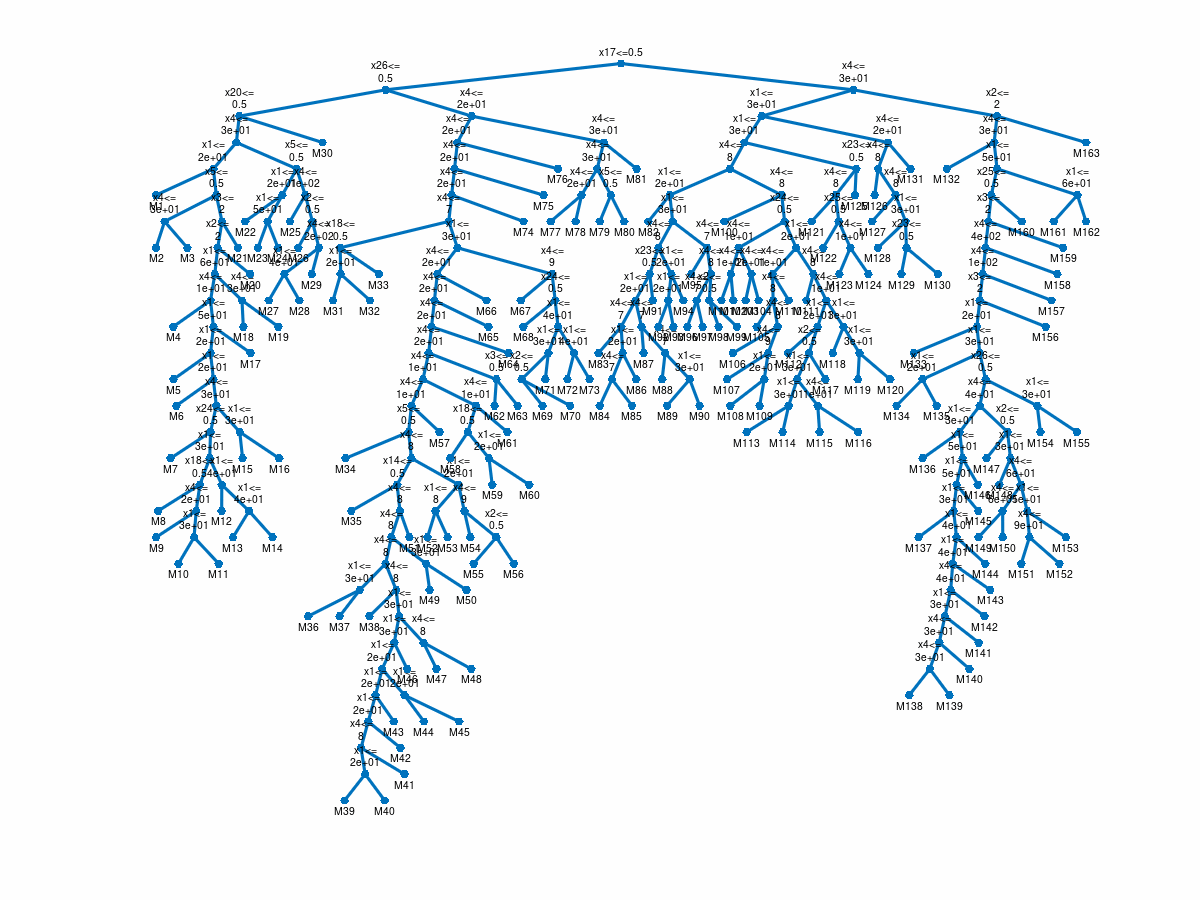
\includegraphics[width=\textwidth,height=\textheight,keepaspectratio]{decision_tree.png}
	\caption{decision tree}
\end{sidewaysfigure}	
\begin{sidewaysfigure}[h]
	\centering
	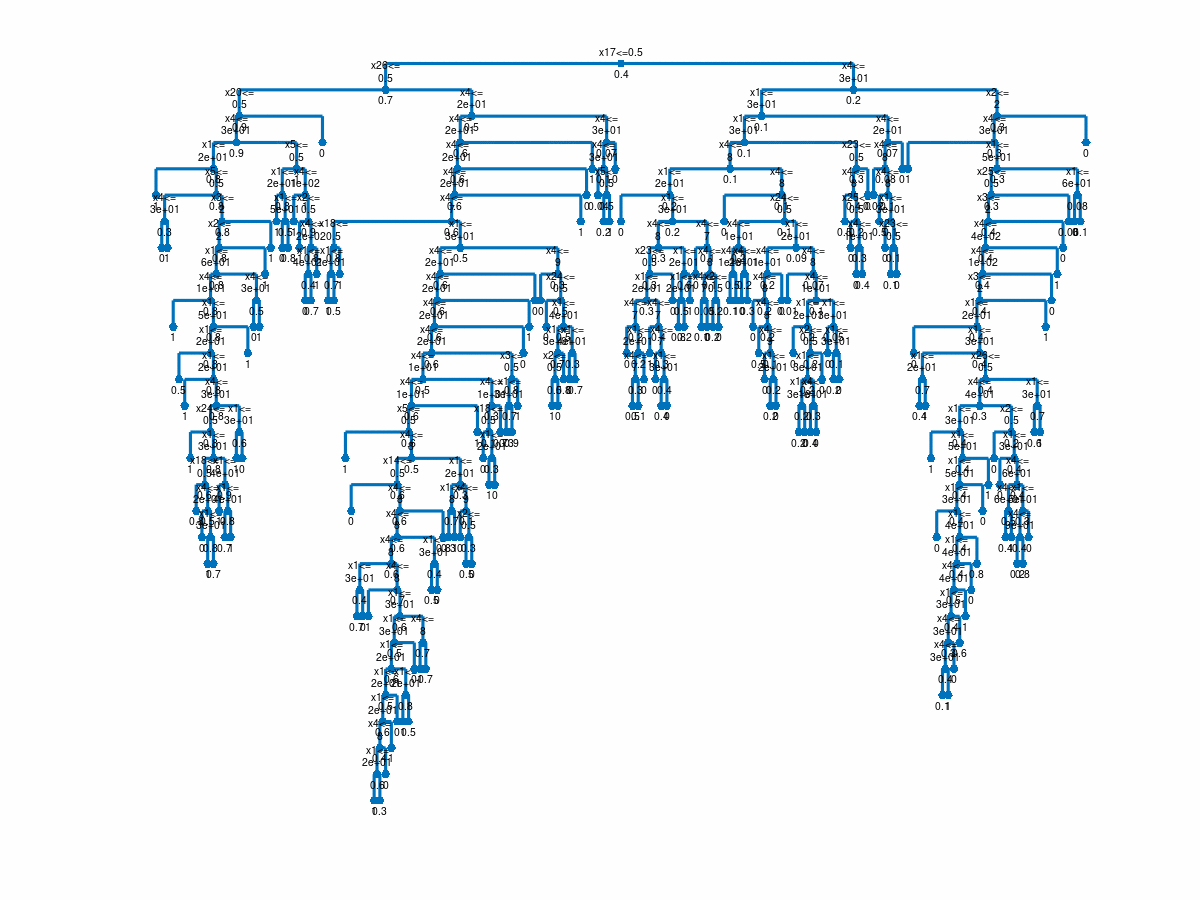
\includegraphics[width=\textwidth,height=\textheight,keepaspectratio]{precision_tree.png}
	\caption{precision tree}
\end{sidewaysfigure}
\vfill
\clearpage

\subsection{Results for Random Forest}
Random forest is grown with 50 trees using Bagging technique. As illustrated the lowest Mean Square Error (MSE) is achieved with 50 trees.
\bigskip
\begin{figure}[H]
	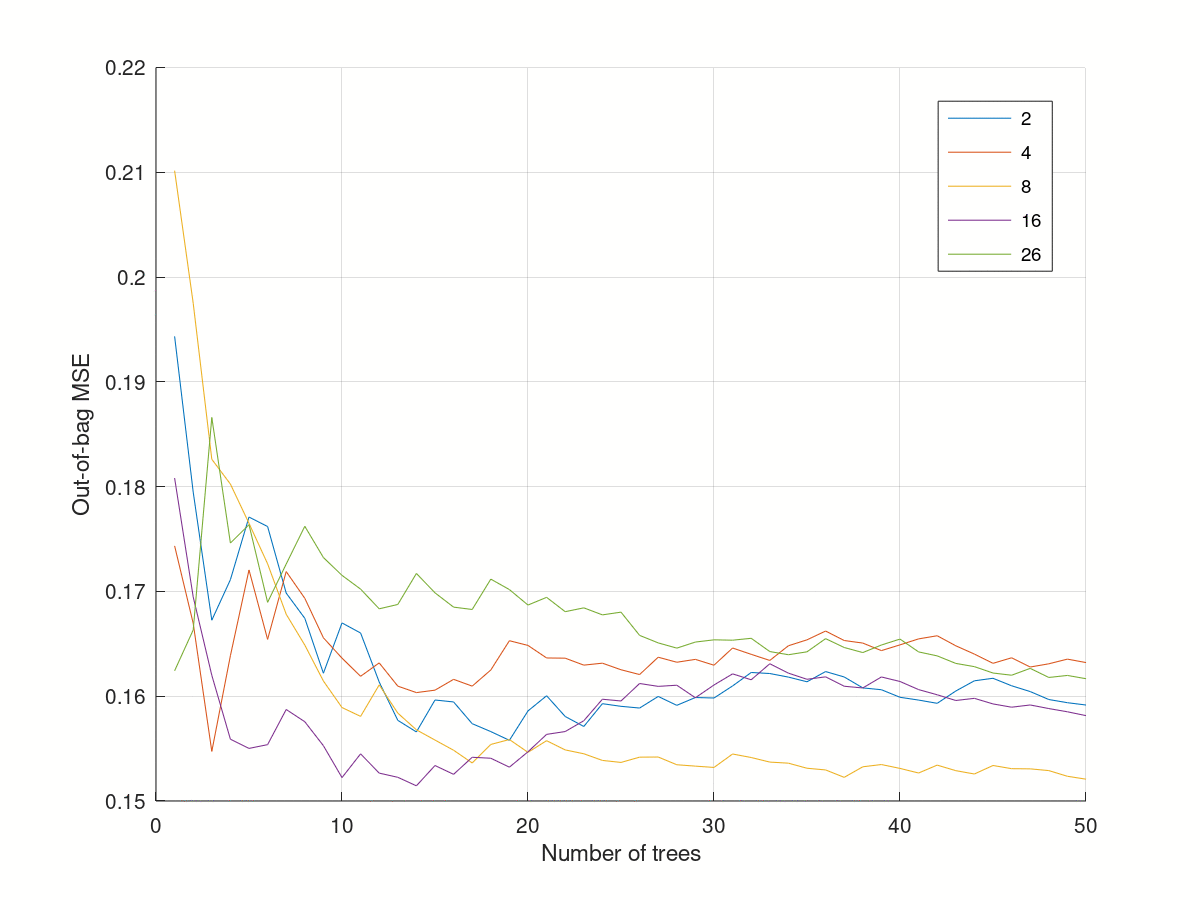
\includegraphics[width=\textwidth,height=\textheight,keepaspectratio]{mse_bagging.png}
	\caption{Out-of-bag MSE using Bagging}
\end{figure}

\begin{figure}[H]
	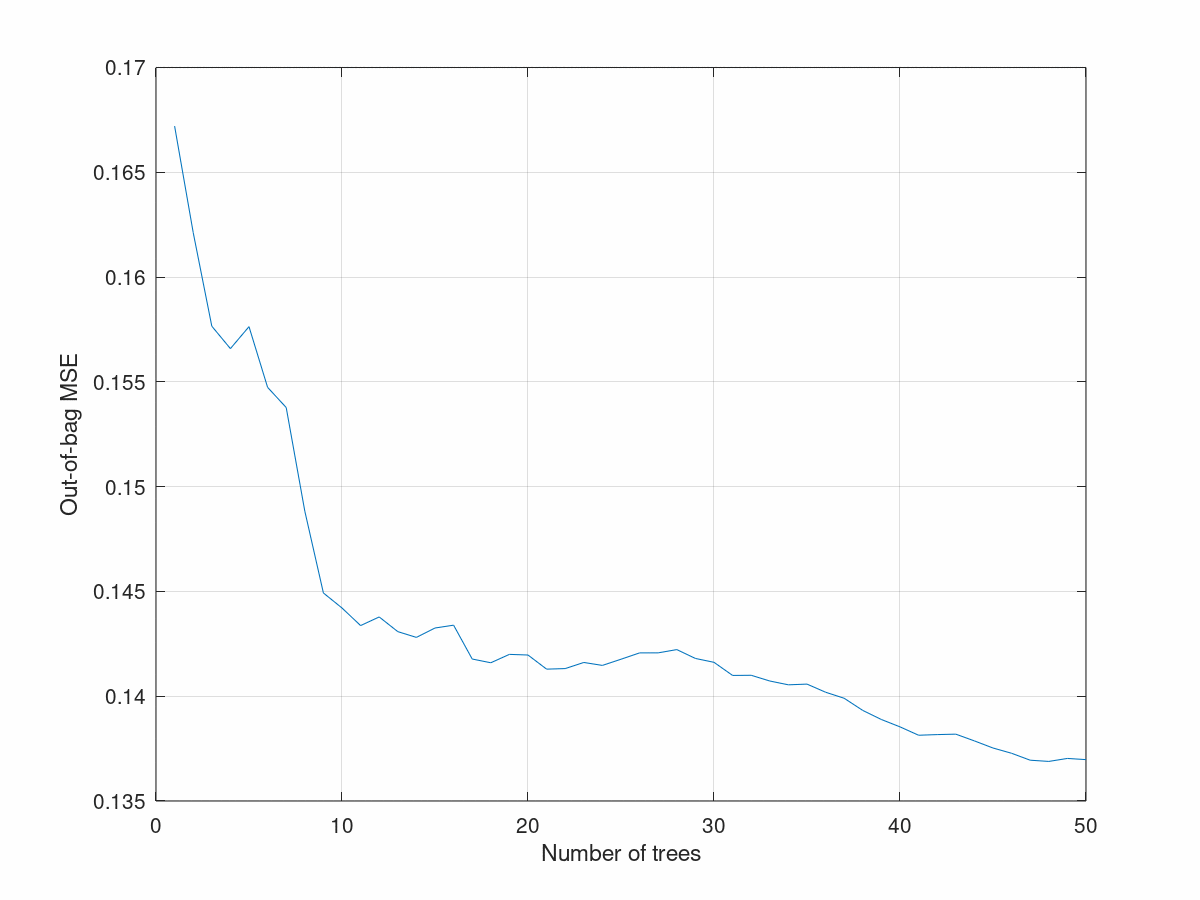
\includegraphics[width=\textwidth,height=\textheight,keepaspectratio]{mse.png}
	\caption{Out-of-bag MSE}
\end{figure}

\begin{figure}[H]
	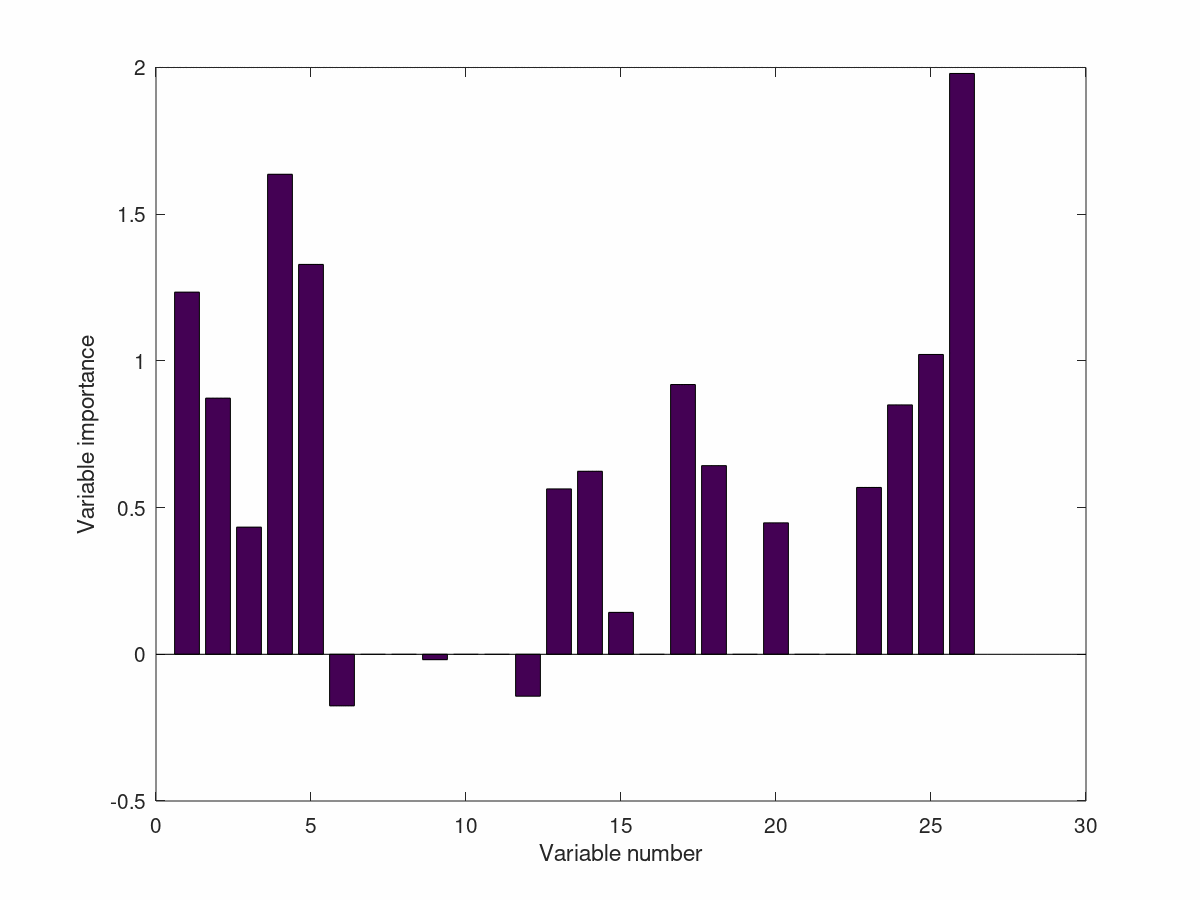
\includegraphics[width=\textwidth,height=\textheight,keepaspectratio]{var_importance.png}
	\caption{Variable importance}
\end{figure}

\begin{figure}[H]
	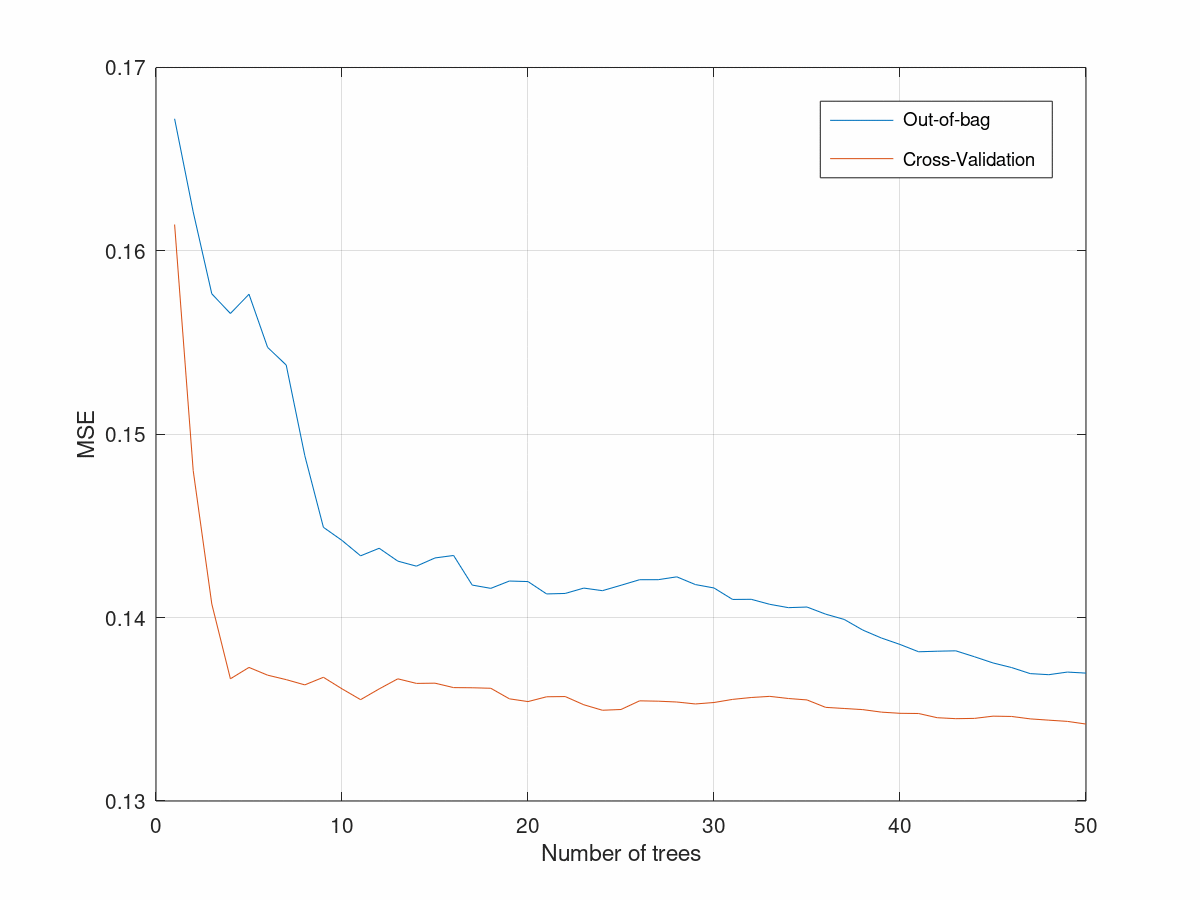
\includegraphics[width=\textwidth,height=\textheight,keepaspectratio]{bag_vs_cv.png}
	\caption{Out-of-bag MSE vs Cross Validation}
\end{figure}

	
\subsection{Lesson learned}
\subsubsection{Advantages of Decision Trees}
\begin{itemize}
	\item No normalization or scaling of features
	\item Suitable for mixed feature data types
	\item Easy results interpretation
\end{itemize}
\subsubsection{Disadvantages of Decision Trees}
\begin{itemize}
\item Prone to overfit and need to build forests to get good results
\end{itemize}

\subsubsection{Advantages of Random Forests}
\begin{itemize}
	\item Same as Random Trees
	\item Powerful, parallel computation and suitable for many different problems
\end{itemize}
\subsubsection{Disadvantages of Random Forests}
\begin{itemize}
	\item Scalability problem with high-dimensional data
\end{itemize}

\section{Naive Bayes Classifier}
A Naive Bayes classifier is a probabilistic machine learning model that’s used for classification task. The classifier is based on the probabilistic Bayes theorem.
\begin{equation}
\label{eq:bayes-theorem}
P(A|B) = \frac{P(B|A) P(A)}{P(B)}
\end{equation}
Using Bayes theorem, we can find the probability of A happening, given that B has occurred. Here, B is the evidence and A is the hypothesis. The assumption made here is that the predictors/features are independent. That is presence of one particular feature does not affect the other. Hence it is called naive.

\subsection{Types of classifier}
\begin{itemize}
	\item Multinomial Naive Bayes: for document classification
	\item Bernoulli Naive Bayes: similar to Multinomial using boolean variables
	\item Gaussian Naive Bayes: for datasets with continuous features
\end{itemize}

\subsection{Results}
\begin{figure}[H]
	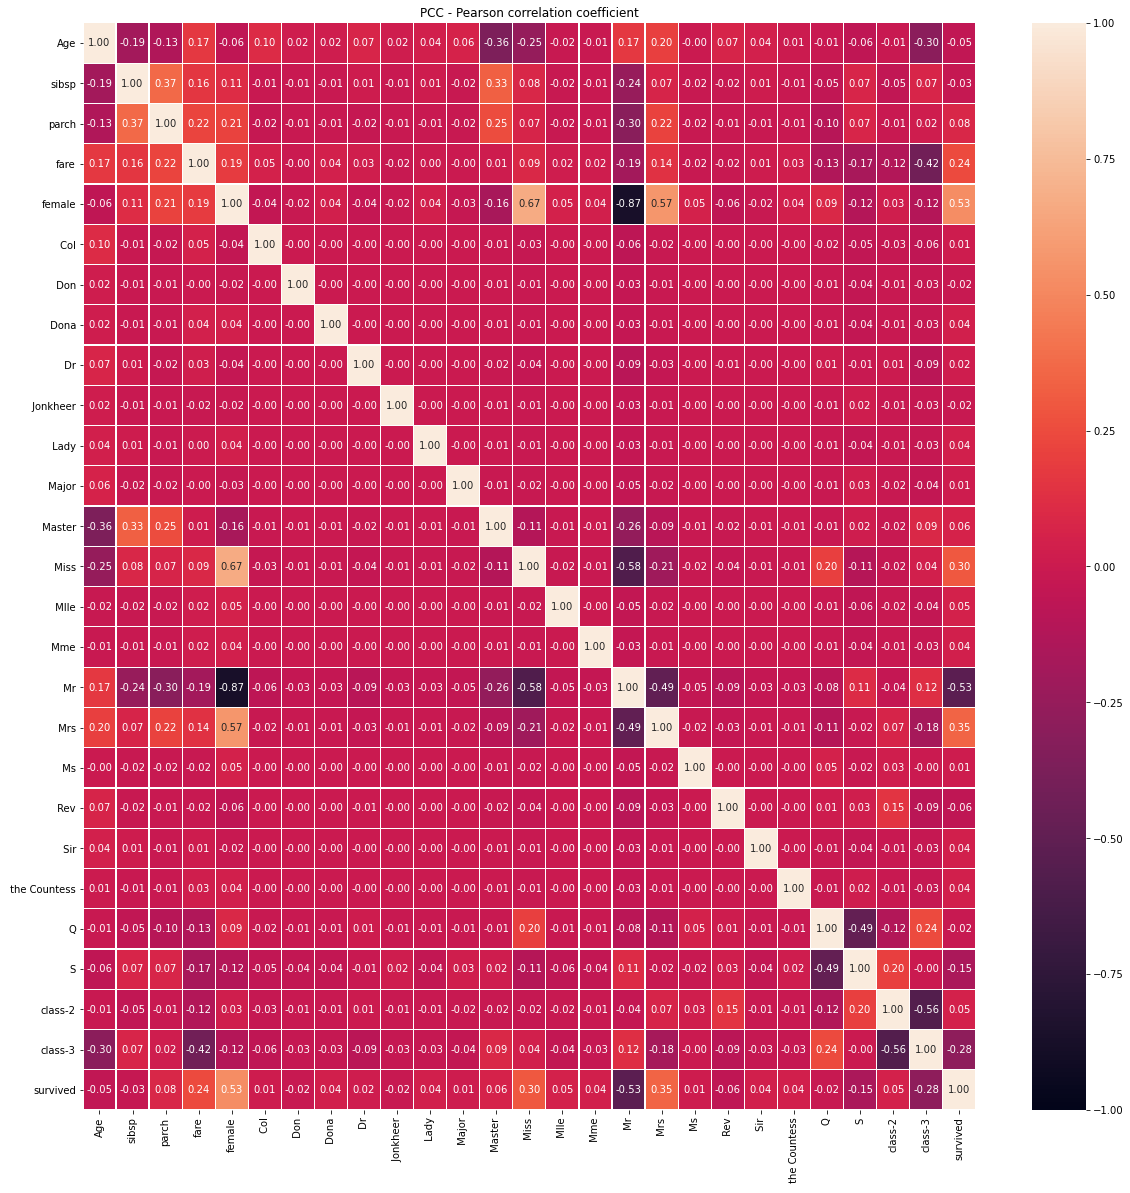
\includegraphics[width=\textwidth,height=\textheight,keepaspectratio]{heat_map.png}
	\caption{PCC - Pearson correlation coefficient}
\end{figure}

\begin{table}[H]
	\centering
	\caption{Model metrics}
	\label{tab:NB-metrics}
	\begin{tabular}{|l|l|l|}
		\hline
		\textbf{Measure} & \textbf{Train} & \textbf{Validation} \\ \hline
		Accuracy       	 & 0.79    & 0.83 \\ \hline
		Recall    		 & 0.71    & 0.82 \\ \hline
		Precision    	 & 0.75    & 0.75 \\ \hline
	\end{tabular}
\end{table}

\begin{table}[H]
	\centering
	\caption{Probability of each class}
	\label{tab:NB-probabilities}
	\begin{tabular}{|l|l|}
		\hline
		\textbf{Measure} & \textbf{Value} \\ \hline
		Survive  = 0     & 0.62    \\ \hline
		Survive  = 1     & 0.38   \\ \hline
	\end{tabular}
\end{table}

\subsection{Lesson learned}
\subsubsection{Advantages}
\begin{itemize}
	\item Fast and easy to implement
\end{itemize}
\subsubsection{Disadvantages}
\begin{itemize}
	\item Features have to be independent for good classifier performance
\end{itemize}


\section{Neural Network}
skt-learn was used 

\subsubsection{Procedure}

\begin{enumerate}
	\item The optimal, from the perspective of accuracy, number of nodes and the number of hidden layers has to be found. A CV based test battery has been set in order. It takes in consideration form 1 to 5 hidden layers and from 22 to 32 nodes per layer. As it can be seen in \ref{tab:sklearn-NoScaling} the best on has 2 hidden layers and 28 nodes per layer, achieves 0.813 accuracy. Do note that the library chosen already applies regularization.
	
	\item One feature that is provided by sklearn is scaling. i.e. data is scaled to have a mean of 0 and std of 1. The methods used are said to improve with the scaling. Another test battery was performed similar to step 1. This time with the feature added. The accuracies estimated have a much smaller variance as it can be noticed in table \ref{tab:Scaled_gradient} in comparison to  \ref{tab:sklearn-NoScaling}.
	
	\item Driven by curiosity another test battery was set up. This battery tries to check for 1-2 hidden layers from 1 to 10 nodes each. The results is very interesting, seen in \ref{tab:NN-LessNodesPerLayer}. One layer with 3 nodes is to be enough to come very close to the accuracy given by 2 hideen layers and 28 nodes. The best model in this range is two layers and 10 nodes. The one found in step 1 is still slightly better.
	
	\item The learning curves can be seen here \ref{PLACE_GRAPH_} . As it can be seen the non-scaled version is much less "smooth" but much faster. It could be based on the simplification of having a lot of 0 values in the data. The result with the same amount of data leads to a less accurate model.
	
\end{enumerate}


Without scaling the module reached the limit of 200 execution. And the values
were not optimal: 
Thesere the results 

\begin{table}[]
\caption{Rows = num hidden layers, Columns = size of hidden layers. Without scaling.}
\label{tab:sklearn-NoScaling}
\begin{tabular}{|l|l|l|l|l|l|l|l|l|l|l|l|}
\hline
           & 22       & 23       & 24       & 25       & 26       & 27       & \textbf{28}       & 29       & 30       & 31       & 32       \\ \hline
1          & 0.618 & 0.781 & 0.809 & 0.649 & 0.382 & 0.618 & 0.358          & 0.812 & 0.618 & 0.618 & 0.772 \\ \hline
\textbf{2} & 0.386 & 0.327 & 0.618 & 0.794 & 0.807 & 0.618 & \textbf{0.813} & 0.58 & 0.809 & 0.322 & 0.458 \\ \hline
3          & 0.618 & 0.79 & 0.455 & 0.793 & 0.616 & 0.618 & 0.798          & 0.336 & 0.618 & 0.618 & 0.618 \\ \hline
4          & 0.760 & 0.805 & 0.5 & 0.780 & 0.614 & 0.618 & 0.803          & 0.612 & 0.803 & 0.618 & 0.804 \\ \hline
5          & 0.6180 & 0.753 & 0.78 & 0.793 & 0.801 & 0.574 & 0.778          & 0.369 & 0.804 & 0.626 & 0.8 \\ \hline
\end{tabular}
\end{table}


\begin{table}[]
\caption{Attempt at using from 1 to 5 hidden layers and from 21 to 31 for the number of nodes in the layers. Using stocastic gradient descent and took 20 min of execution.
The most  accurate model is 2 hidden layers and 28 nodes each}
\label{tab:Scaled_gradient}
\begin{tabular}{|l|l|l|l|l|l|l|l|l|l|l|l|}
\hline
           & 21    & 22    & 23    & 24    & 25    & 26    & 27    & \textbf{28}    & 29    & 30    & 31    \\ \hline
1          & 0.802 & 0.812 & 0.806 & 0.802 & 0.799 & 0.81  & 0.807 & 0.811          & 0.805 & 0.802 & 0.81  \\ \hline
\textbf{2} & 0.806 & 0.804 & 0.806 & 0.811 & 0.803 & 0.812 & 0.804 & \textbf{0.814} & 0.807 & 0.807 & 0.806 \\ \hline
3          & 0.802 & 0.803 & 0.807 & 0.802 & 0.805 & 0.802 & 0.802 & 0.811          & 0.806 & 0.811 & 0.798 \\ \hline
4          & 0.807 & 0.801 & 0.807 & 0.807 & 0.807 & 0.807 & 0.801 & 0.804          & 0.796 & 0.807 & 0.806 \\ \hline
5          & 0.801 & 0.798 & 0.797 & 0.803 & 0.803 & 0.804 & 0.803 & 0.801          & 0.804 & 0.805 & 0.801 \\ \hline
\end{tabular}
\end{table}


\begin{table}[]
\caption{Check for precision with less nodes per layer. Using only 1 or 2 layers. From 1 to 20 nodes. The best model in this range is 2 hidden layers with 10 nodes. But 1 single layer with 3 nodes also behaves very well while being much more simple.}
\label{tab:NN-LessNodesPerLayer}
\begin{tabular}{|l|l|l|l|l|l|l|l|l|l|l|l|l|l|l|l|l|l|l|l|l|}
\hline
           & 1     & 2     & 3              & 4     & 5     & 6     & 7     & 8     & 9     & \textbf{10}    & 11    & 12    & 13    & 14    & 15    & 16    & 17    & 18    & 19    & 20    \\ \hline
1          & 0.769 & 0.791 & \textbf{0.810} & 0.787 & 0.799 & 0.800 & 0.804 & 0.807 & 0.804 & 0.804          & 0.807 & 0.807 & 0.805 & 0.807 & 0.808 & 0.810 & 0.807 & 0.808 & 0.801 & 0.807 \\ \hline
\textbf{2} & 0.618 & 0.781 & 0.792          & 0.773 & 0.798 & 0.802 & 0.799 & 0.805 & 0.797 & \textbf{0.812} & 0.799 & 0.808 & 0.805 & 0.805 & 0.809 & 0.804 & 0.801 & 0.804 & 0.804 & 0.804 \\ \hline
\end{tabular}
\end{table}

\section{Conclusion}
Write your conclusion here.

\end{document}

